\chapter{Results on Synthetic Data} \label{chap:ResultsSynData}

This chapter presents the major results of this thesis. First, an optimal blending pattern for simultaneous crossline sources will be derived. Then, the advantages of a 3D $f$-$k_x$-$k_y$-filter towards a 2D $f$-$k$-filter will be shown. Finally, the feasibility of the suggested acquisition design will be proven on a synthetic 3D data set. 
 
\section{Blending pattern}

\begin{comment}
\begin{itemize}
	\item Explain how the acquisition limits the firing pattern
	\item Introduce spatial incoherency
	\item Suggest the applied blending pattern
	\item Show quality factor versus incoherency/firing pattern
\end{itemize}
\end{comment}

An incoherent blending pattern is crucial for good deblending performance (see section \ref{sec:BlendingMatrix}). Thus, a measure of incoherency and deblending quality will be introduced. Then, the possibilities of creating an incoherent blending pattern are presented. Finally, the effect of incoherency and of the maximum firing time delay on the deblending performance will be demonstrated.

\subsection*{Incoherency Measure}

In this thesis only the incoherency of the acquisition design is considered. Thus, the blending matrix, $\Gamma$, or more precisely the product $\mathbf{\Gamma \Gamma}^H$ determines the incoherency.

In section \ref{sec:BlendingMatrix} it was shown that for an incoherent blending pattern the elements, $\mathrm{e}^{-j \omega \Delta t_{kl}}$, along a sub-diagonal of the product $\mathbf{\Gamma \Gamma}^H$ should be out of phase. Therefore, the phase variability of the sub-diagonal elements will be used to quantify incoherency.

Note that the sub-diagonal elements, $\mathrm{e}^{-j \omega \Delta t_{kl}}$, map in the complex plane on a circle with radius 1 (see Figure \ref{fig:Ch-Results-complex-circle}). 

\begin{figure}
	\centering
	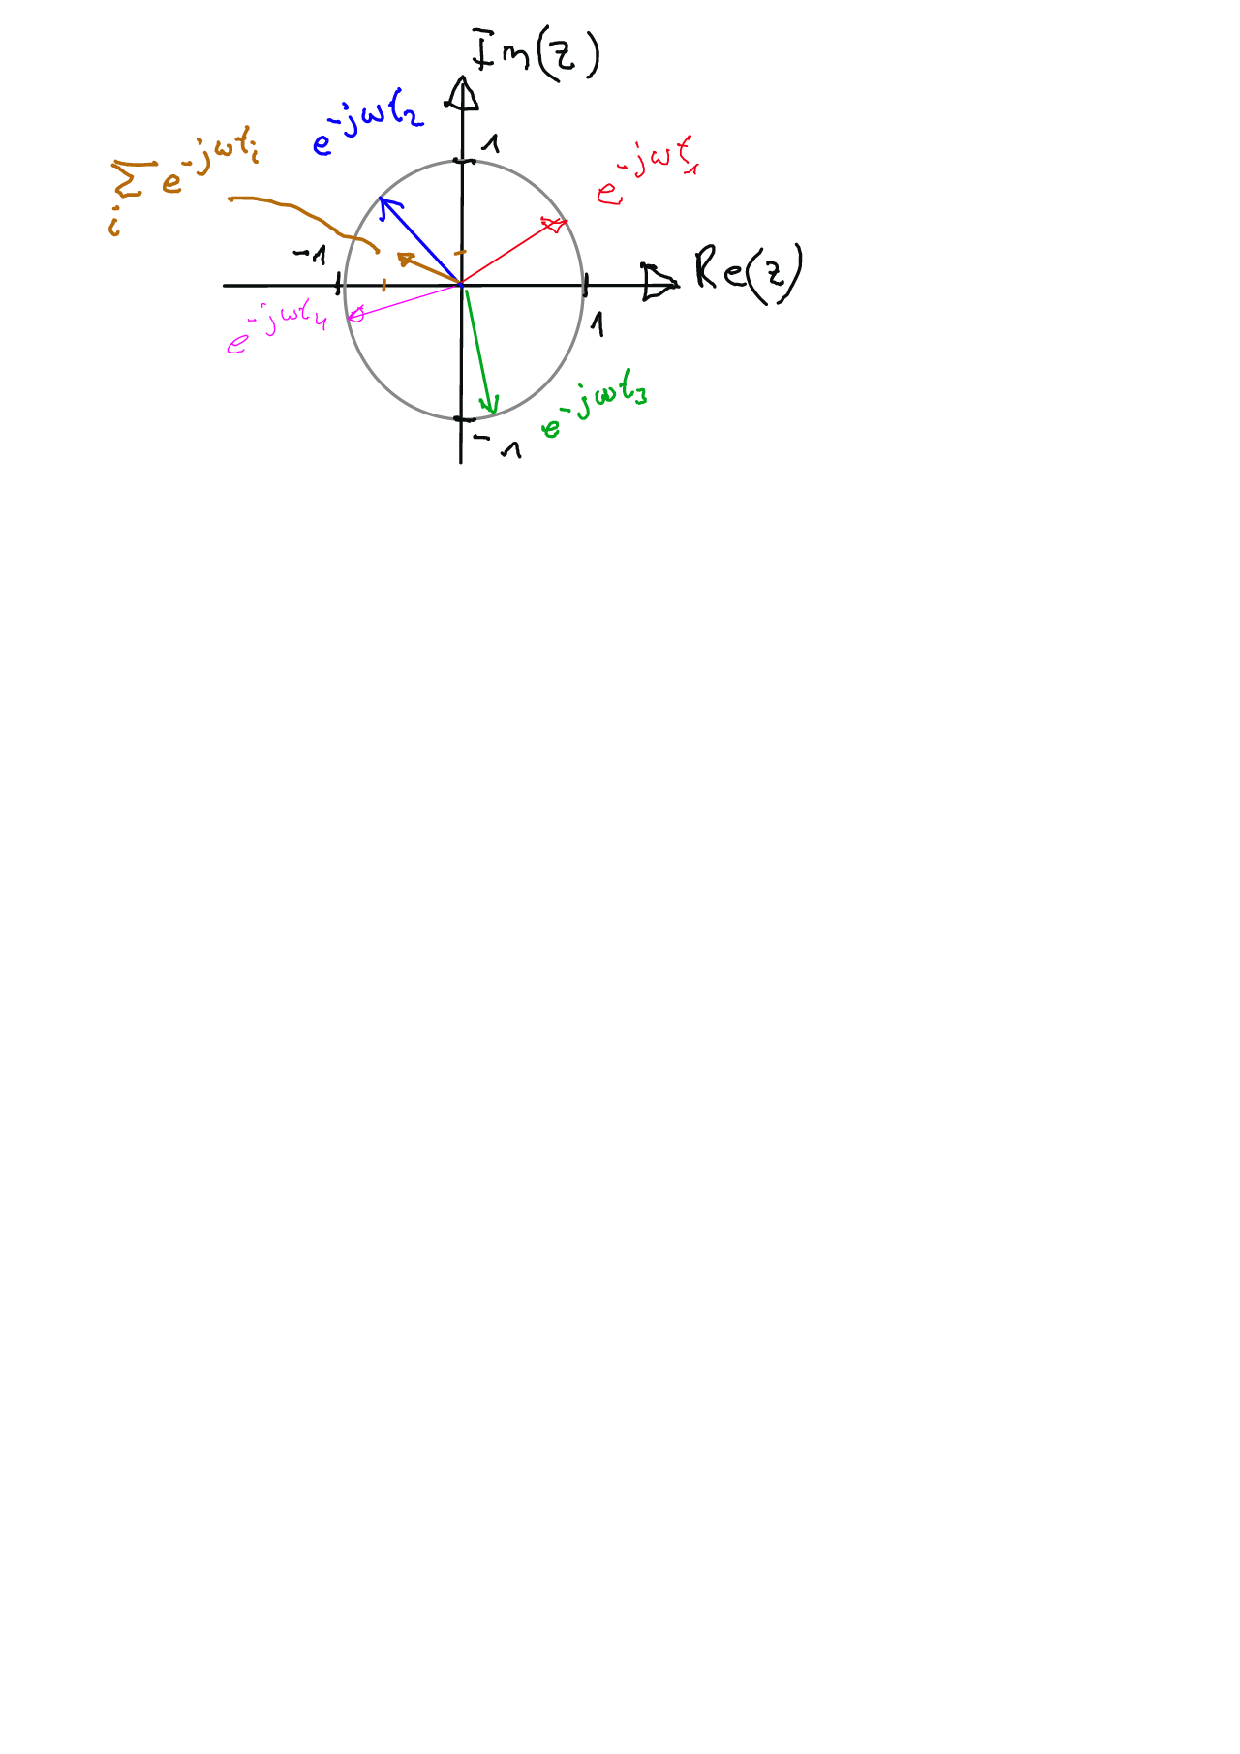
\includegraphics[width = 0.5\textwidth]{Plots/complex-circle}
	\caption{Illustration of the sub-diagonal elements in the complex number plane. The elements have unit length and variable phase. The absolute value of their sum depends on the phase coherency of the elements.}
	\label{fig:Ch-Results-complex-circle}
\end{figure}

The sum of the elements along the $k^{th}$ sub-diagonal can be constructive or destructive, depending on the phase variability. Thus, the absolute value of the sum measures the incoherency of an individual sub-diagonal. The resulting value is squared in order to put it in terms of energy;

\begin{equation}
	\left| \sum_{j-i=k} \mathbf{\Gamma \Gamma}^H_{ij} (\omega) \right|^2.
	\label{eq:Ch-Results-incoherency-diagsum}	
\end{equation} 

For example, if all elements are in phase the length of their sum is maximized. The more the elements are out of phase, i.e. the more incoherent they are, the smaller is the length of the summed elements. 

For illustration a blending matrix, $\mathbf{\Gamma}$, is generated and inserted in equation \ref{eq:Ch-Results-incoherency-diagsum}. This yields an output for each sub-diagonal, which is shown in Figure \ref{fig:Ch-Results-Diagonal-Sums}. The spike is caused by the elements on the main diagonal of $\mathbf{\Gamma \Gamma}^H$, which are all equal to 1, i.e. in phase. For a perfectly incoherent blending design the elements on a sub-diagonal cancel and the plot becomes a perfect spike. 


\begin{figure}
	\centering
	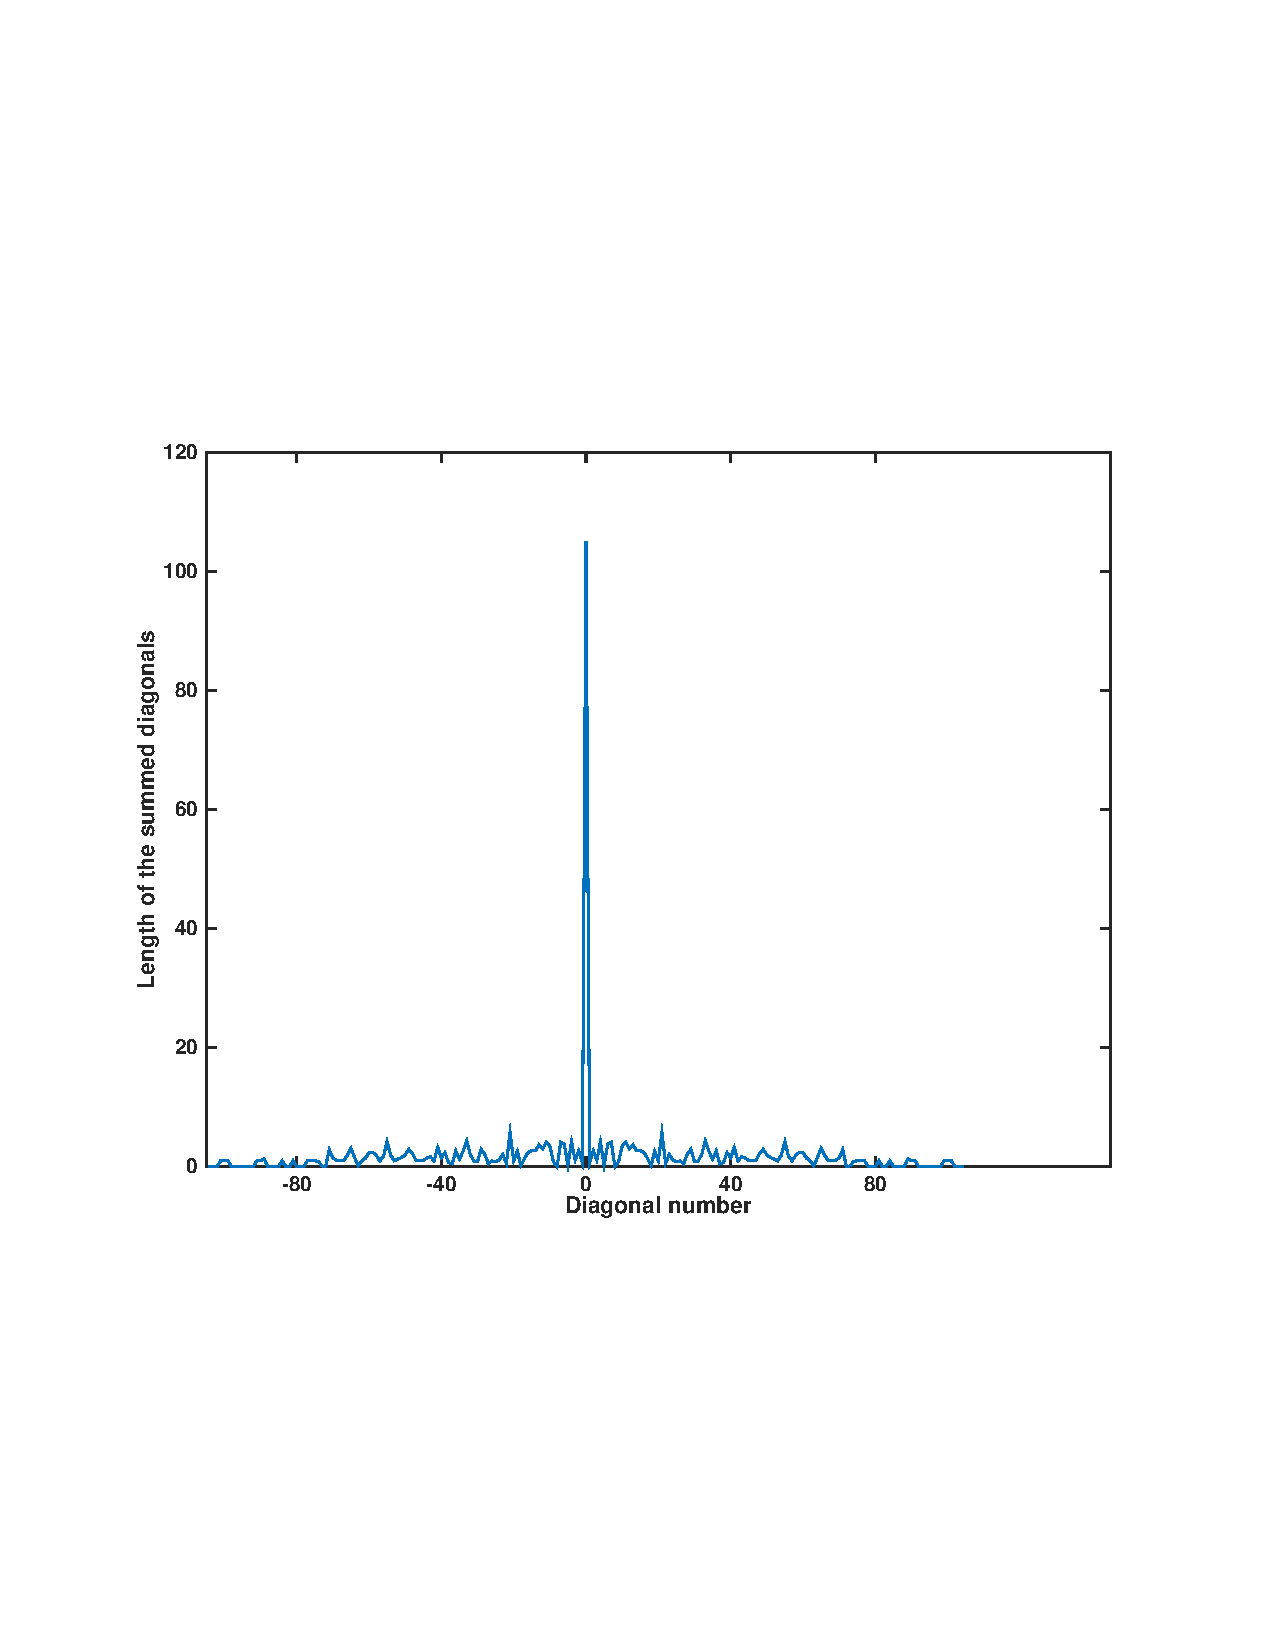
\includegraphics[width=0.6\textwidth]{Plots/diagonal-sums}
	\caption{The sub-diagonal elements, $\mathrm{e}^{-j \omega \Delta t_{kl}}$, of the product $\mathbf{\Gamma \Gamma}^H$ are summed. The length of each output is plotted. The spike is caused by the main diagonal elements of $\mathbf{\Gamma \Gamma}^H$ because they are all in phase.}
	\label{fig:Ch-Results-Diagonal-Sums}
\end{figure}

The closer Figure \ref{fig:Ch-Results-Diagonal-Sums} comes to a spike the more incoherent is the blending pattern. Thus, considering Figure \ref{fig:Ch-Results-Diagonal-Sums} the incoherency, $\mu$, is measured as the ratio between the amplitude of the spike and the sum of all amplitudes. 

In terms of the sub-diagonals of $\mathbf{\Gamma \Gamma}^H$ this is the ratio between the squared absolute value of the summed main diagonal and the sum of all squared absolute summed sub-diagonals;

\begin{equation}
	\mu(\omega) = \frac{  \left| \sum_{j-i = 0} \mathbf{\Gamma \Gamma}^H_{ij} (\omega) \right|^2    }{ \sum_{k = 1-N_s}^{N_s-1}	 \left( \left| \sum_{j-i = k} \mathbf{\Gamma \Gamma}^H_{ij} (\omega) \right|^2 \right)   }.
	\label{eq:Ch-Results-incoherency-monochromatic}
\end{equation}

Note that $N_s$ is the number of sources, i.e. the matrix $\mathbf{\Gamma \Gamma}^H$ has $N_s$ rows and columns.

Up to now, the incoherency is computed for each frequency separately. In order to account for all frequencies at once the nominator and denominator in equation \ref{eq:Ch-Results-incoherency-monochromatic} are summed over all frequency components;

\begin{equation}
	\mu = \frac{  \sum_{\omega} \left( \left| \sum_{j-i = 0} \mathbf{\Gamma \Gamma}^H_{ij} (\omega) \right|^2  \right)  }{  \sum_{\omega} \left( \sum_{k = 1-N_s}^{N_s-1}	 \left( \left| \sum_{j-i = k} \mathbf{\Gamma \Gamma}^H_{ij} (\omega) \right|^2 \right) \right)  } \;.
	\label{eq:Ch-Results-incoherency}
\end{equation}



For example, for a perfectly incoherent blending pattern only the sum along the main diagonal ($k=0$) is non zero. Thus, the nominator and the denominator in equation \ref{eq:Ch-Results-incoherency} are identical, the incoherency equals 1. 

In contrast, for a perfectly coherent blending pattern all sub-diagonal elements are in phase. Consequently, the sum along the main diagonal is of the same magnitude as the sum along the sub-diagonals. The nominator in equation \ref{eq:Ch-Results-incoherency} becomes significantly smaller than the denominator, and the incoherency is nearly 0.



\subsection*{Deblending Performance Measure}

The following data examples are synthetic data, i.e. the unblended data is known. Therefore, the deblending performance can be measured with the quality factor, $Q$, which is defined by \citet{IbrahimQuality} as;

\begin{equation}
	Q = 10 \cdot \mathrm{log_{10}} \left( \frac{\left|\left|\text{Unblended data}\right|\right| _2 ^2}{\left|\left|\text{Unblended data - Deblended data}\right|\right| _2 ^2} \right) \;.	
\end{equation}



\subsection*{Incoherent Blending Patterns}

This thesis considers the following blended acquisition set up: The sources are assembled in crossline direction and move towards inline direction due to the vessel movement (see Figure \ref{fig:Ch-Theory-3D-BlendedAcquisition}). As a consequence each experiment can blend sources which belong to the same crossline. The inline source sampling rate must be sufficiently small to avoid spatial aliasing. Thus, the sources within one crossline must be blended and recorded before the vessel reaches the next inline position.

Based on this set up there are three possibilities to blend the sources incoherently. First, the sources can be blended with random time delays (temporal incoherency). Second, one can randomly pick sources for each experiment (spatial incoherency). Third, temporal and spatial incoherency can be combined (mixed incoherency), i.e. randomly picked sources are blended with random time delays.

In the following these blending patterns will applied to a synthetic data set (see Figure \ref{fig:Ch-Results-Unbl-Delphi}, \ref{fig:Ch-Results-Unbl-inline10}, \ref{fig:Ch-Results-Unbl-xline10}). Next, the data is deblended with the 3D deblending algorithm of chapter \ref{chap:MahdadMethod3d}. 

The deblending results are shown in Figure \ref{fig:Ch-Results-Debl-Delphi} and \ref{fig:Ch-Results-Debl-x-inline}. The results suggest that only spatial incoherency is not sufficient to deblend the data (see Figure \ref{fig:Ch-Results-Debl-Delphi-x}, \ref{fig:Ch-Results-Debl-inline10-x}, \ref{fig:Ch-Results-Debl-xline10-x}). By introducing random firing time delays the deblended data improves significantly as shown in Figure \ref{fig:Ch-Results-Debl-Delphi-t}, \ref{fig:Ch-Results-Debl-inline10-t}, \ref{fig:Ch-Results-Debl-xline10-t}). A combination of both spatial and temporal incoherency enhances the deblended data further (see Figure \ref{fig:Ch-Results-Debl-Delphi-xt}, \ref{fig:Ch-Results-Debl-inline10-xt}, \ref{fig:Ch-Results-Debl-xline10-xt}).

\begin{figure}
	\centering
	\begin{subfigure}[t]{0.8\textwidth}
		\centering
		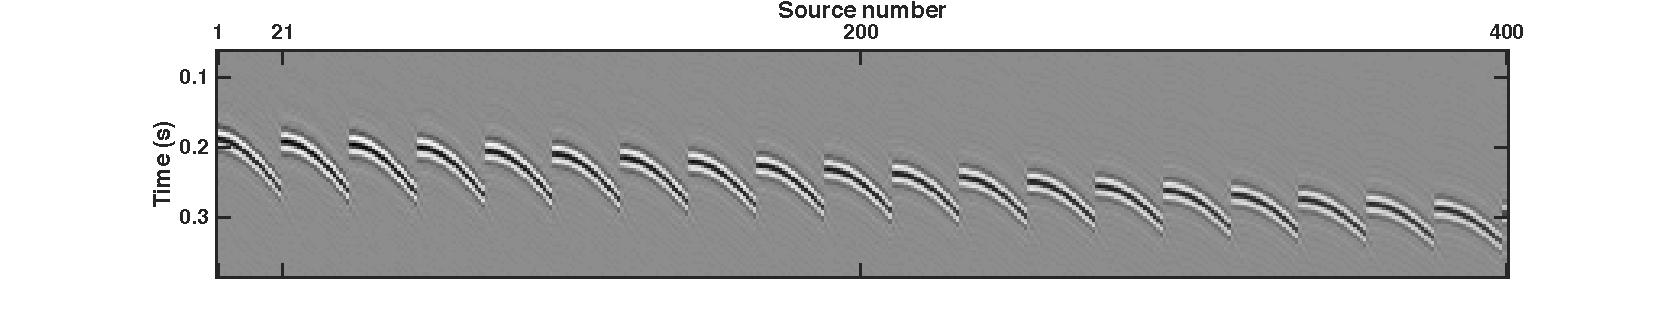
\includegraphics[width = \textwidth]{Plots/BlendingPatterns/Unblended_Delphi_zoom}
		\caption{}
		\label{fig:Ch-Results-Unbl-Delphi}
	\end{subfigure}
	\par\bigskip
	\centering
	\begin{subfigure}[t]{0.8\textwidth}
		\centering
		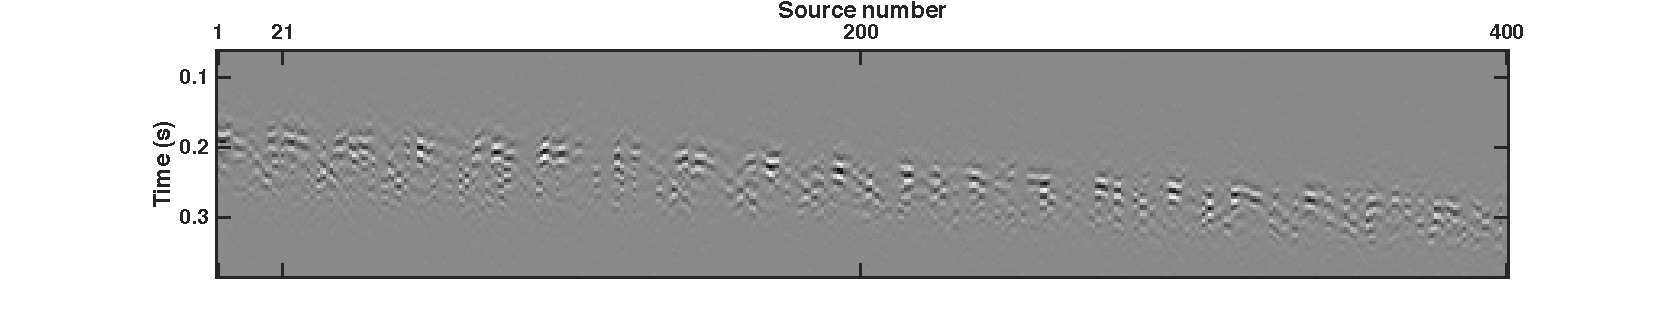
\includegraphics[width = \textwidth]{Plots/BlendingPatterns/Deblended_Delphi_zoomx}
		\caption{}
		\label{fig:Ch-Results-Debl-Delphi-x}
	\end{subfigure}
	\par\bigskip
	\centering
	\begin{subfigure}[t]{0.8\textwidth}
		\centering
		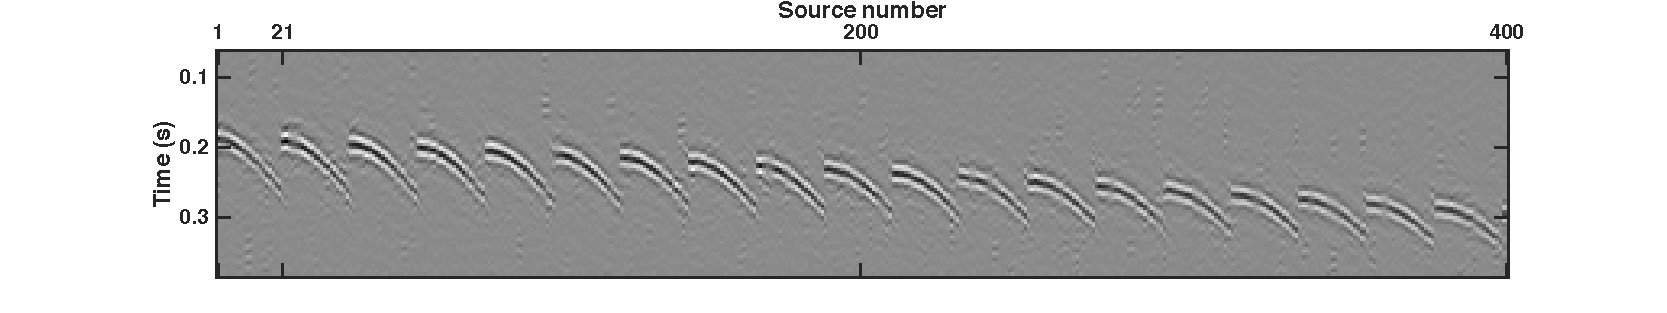
\includegraphics[width = \textwidth]{Plots/BlendingPatterns/Deblended_Delphi_zoomt}
		\caption{}
		\label{fig:Ch-Results-Debl-Delphi-t}
	\end{subfigure}
	\par\bigskip
	\centering
	\begin{subfigure}[t]{0.8\textwidth}
		\centering
		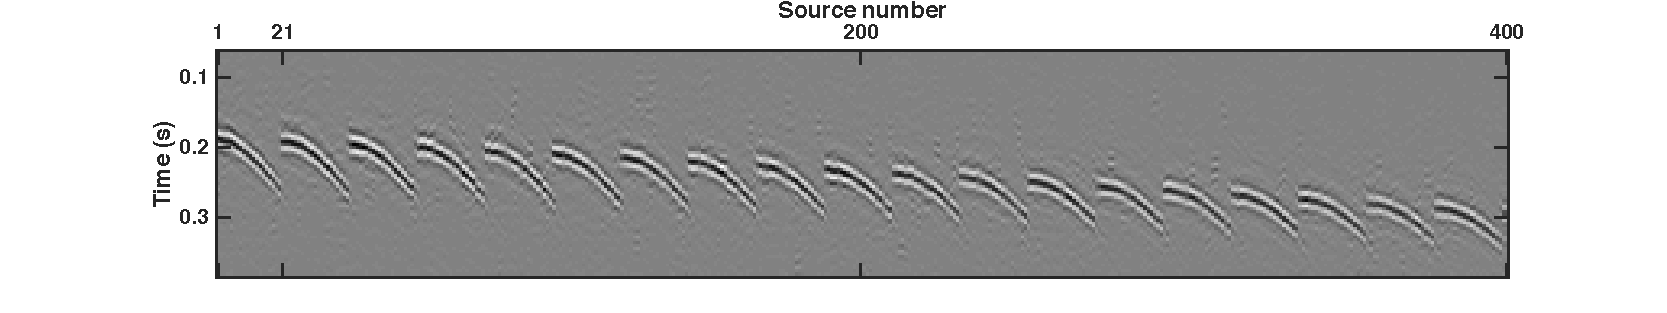
\includegraphics[width = \textwidth]{Plots/BlendingPatterns/Deblended_Delphi_zoomxt}
		\caption{}
		\label{fig:Ch-Results-Debl-Delphi-xt}
	\end{subfigure}
	
	\caption{These 3D common receiver gathers are sorted according to section \ref{sec:Ch-Theory-3dExtension-DataSorting}. The unblended synthetic data (a) is used to simulate a blended acquisition with 3 experiments per crossline and 7 shots per experiment. The maximum firing time delay is \SI{400}{\milli\second}. The sources are blended in three different patterns: (b) Randomly selected sources are blended without time delay, (c) neighboring sources are blended with random time delays, (d) randomly picked sources are blended with random time delays. Next, the blended data sets are deblended. The corresponding deblending results are illustrated in (b) to (d).}
	\label{fig:Ch-Results-Debl-Delphi}
	
\end{figure}

\todo[inline]{Make a sketch of the set up of the synthetic data.}

\begin{figure}
	\centering
	\begin{subfigure}[t]{0.24\textwidth}
		\centering
		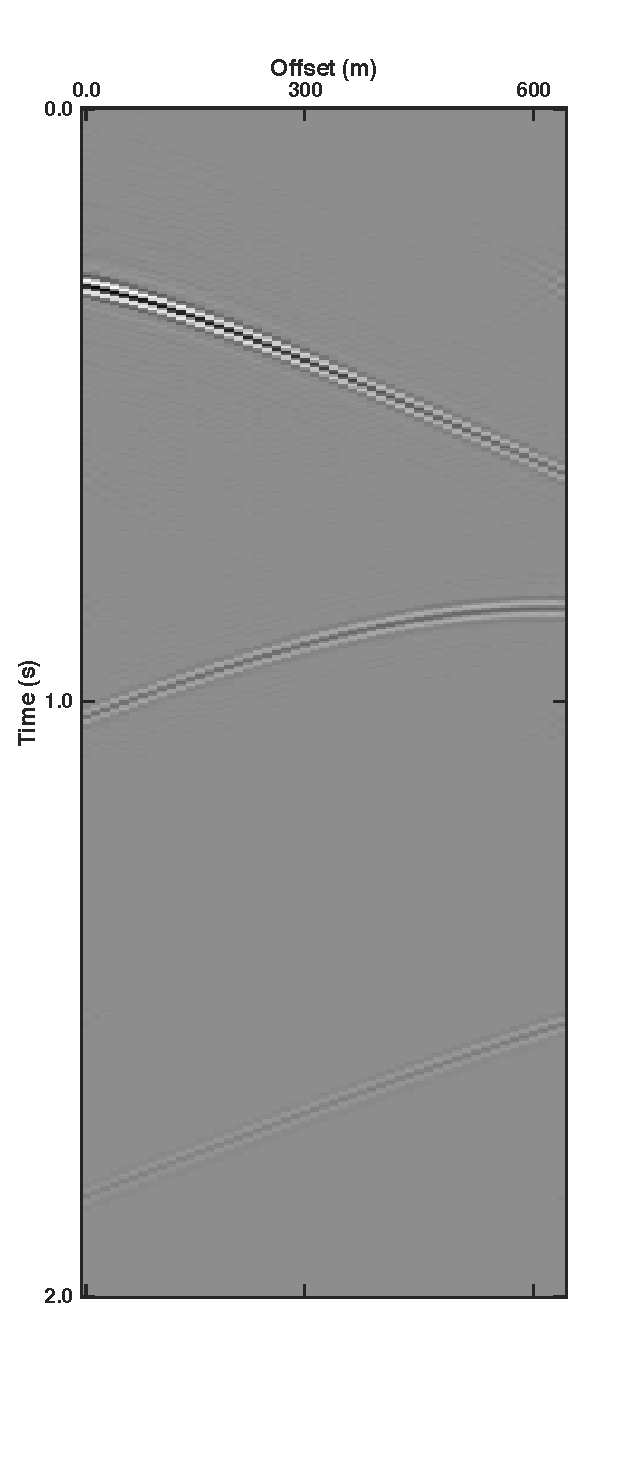
\includegraphics[height = 0.38\textheight]{Plots/BlendingPatterns/Unblended_inline10}
		\caption{}
		\label{fig:Ch-Results-Unbl-inline10}
	\end{subfigure}
	%	
	\centering
	\begin{subfigure}[t]{0.24\textwidth}
		\centering
		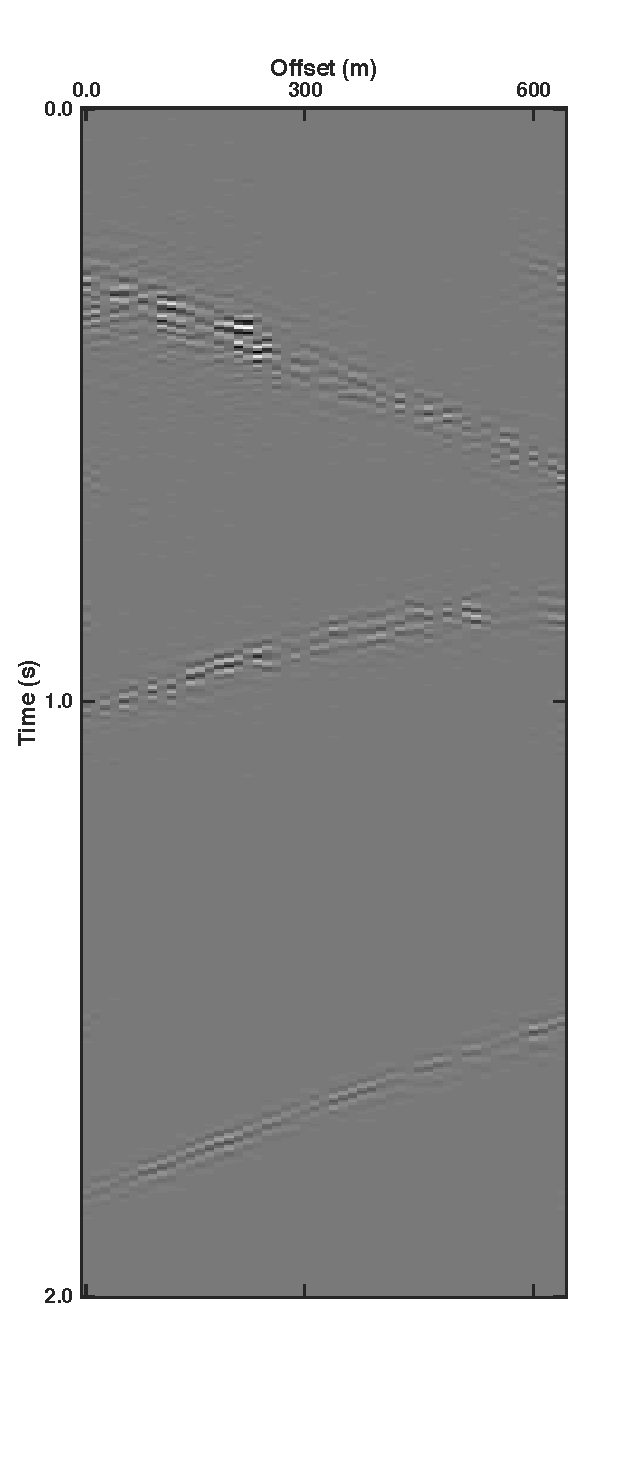
\includegraphics[height = 0.38\textheight]{Plots/BlendingPatterns/Deblended_inline10x}
		\caption{}
		\label{fig:Ch-Results-Debl-inline10-x}
	\end{subfigure}
	%
	\centering
	\begin{subfigure}[t]{0.24\textwidth}
		\centering
		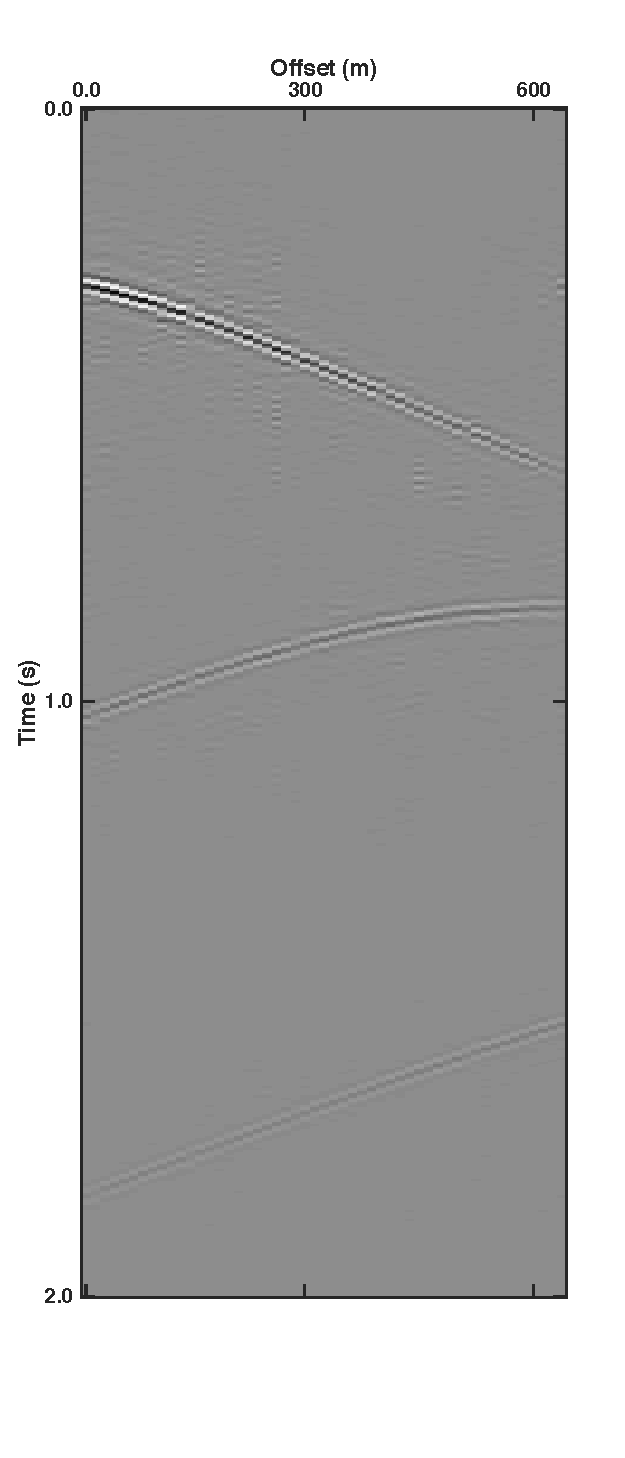
\includegraphics[height = 0.38\textheight]{Plots/BlendingPatterns/Deblended_inline10t}
		\caption{}
		\label{fig:Ch-Results-Debl-inline10-t}
	\end{subfigure}
	%
	\centering
	\begin{subfigure}[t]{0.24\textwidth}
		\centering
		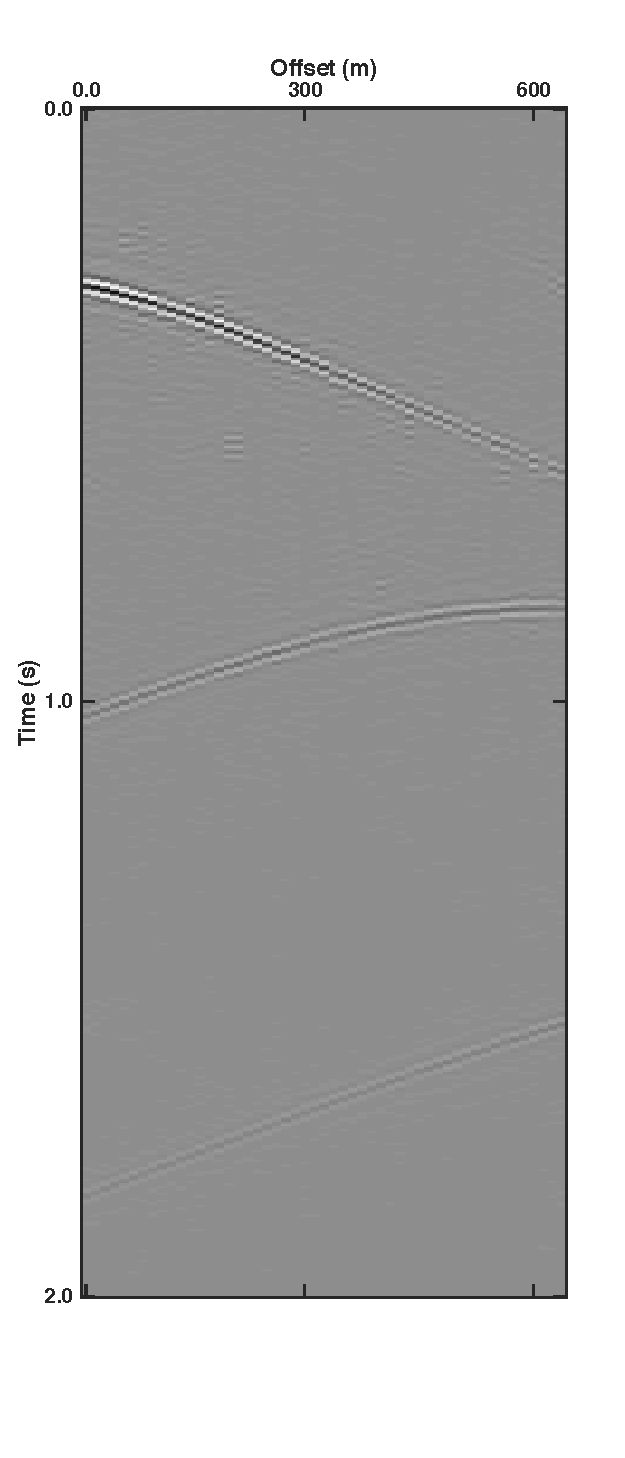
\includegraphics[height = 0.38\textheight]{Plots/BlendingPatterns/Deblended_inline10xt}
		\caption{}
		\label{fig:Ch-Results-Debl-inline10-xt}
	\end{subfigure}
	\par\bigskip
	\centering
	\begin{subfigure}[t]{0.24\textwidth}
		\centering
		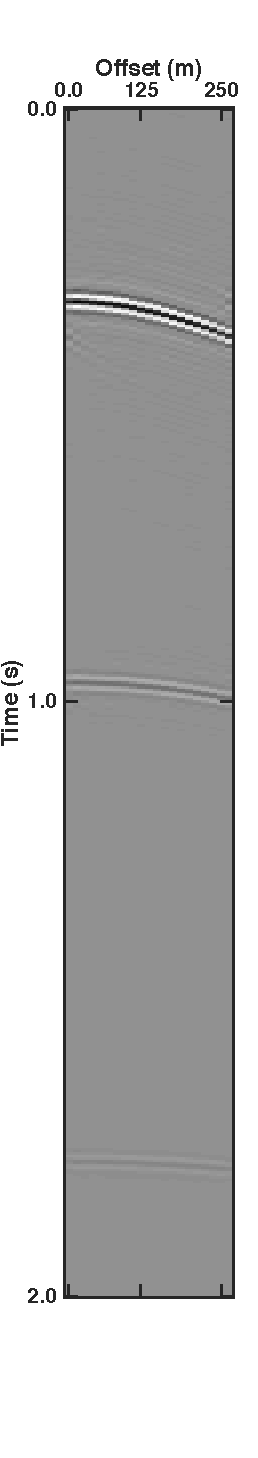
\includegraphics[height = 0.38\textheight]{Plots/BlendingPatterns/Unblended_xline10}
		\caption{}
		\label{fig:Ch-Results-Unbl-xline10}
	\end{subfigure}
	%	
	\centering
	\begin{subfigure}[t]{0.24\textwidth}
		\centering
		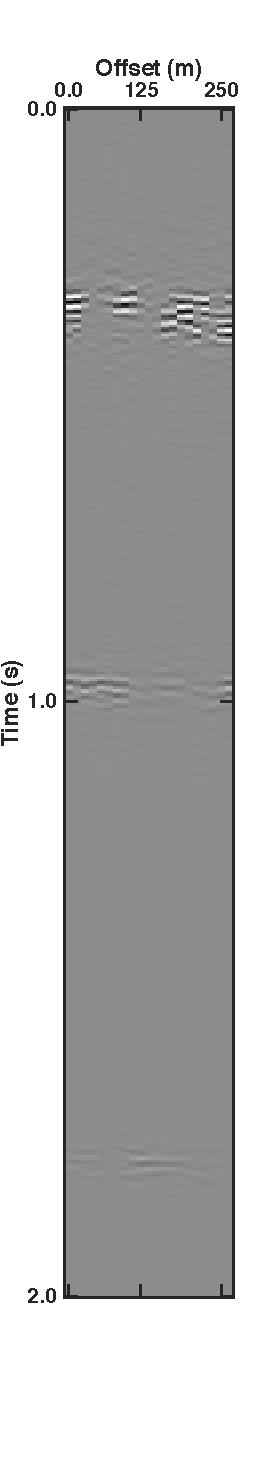
\includegraphics[height = 0.38\textheight]{Plots/BlendingPatterns/Deblended_xline10x}
		\caption{}
		\label{fig:Ch-Results-Debl-xline10-x}
	\end{subfigure}
	%
	\centering
	\begin{subfigure}[t]{0.24\textwidth}
		\centering
		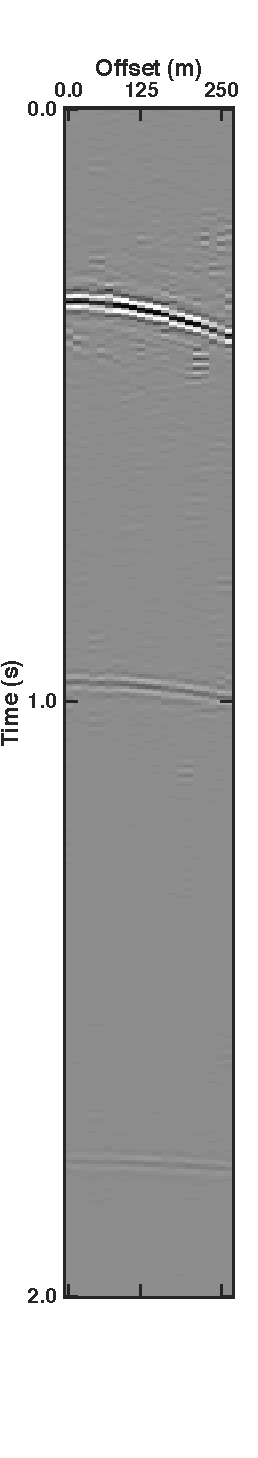
\includegraphics[height = 0.38\textheight]{Plots/BlendingPatterns/Deblended_xline10t}
		\caption{}
		\label{fig:Ch-Results-Debl-xline10-t}
	\end{subfigure}
	%
	\centering
	\begin{subfigure}[t]{0.24\textwidth}
		\centering
		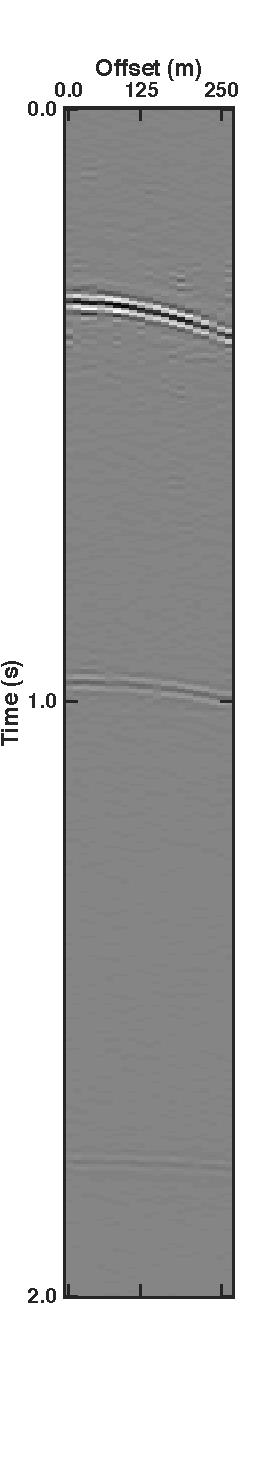
\includegraphics[height = 0.38\textheight]{Plots/BlendingPatterns/Deblended_xline10xt}
		\caption{}
		\label{fig:Ch-Results-Debl-xline10-xt}
	\end{subfigure}
	
	\caption{(a)-(d) show inline slices of the data shown in Figure \ref{fig:Ch-Results-Debl-Delphi}. (e)-(h) display the corresponding crossline slices. }
	\label{fig:Ch-Results-Debl-x-inline}

\end{figure}


\subsection*{Effect of Incoherency}

The above comparison of incoherencies distinguishes different incoherency types. However, each of these types has a different degree of incoherency, $\mu$. Therefore, the dependence of the deblending quality, $Q$, on the incoherency, $\mu$, will be analyzed.

For this purpose blending matrices with incoherencies between \SI{5}{\percent} and \SI{100}{\percent} are generated. Next, synthetic data is blended and deblended with these blending matrices. The quality factor, $Q$, is computed for each deblended data set. Figure \ref{fig:Ch-Results-QvsMu} illustrates the resulting quality factor as a function of the incoherency. 

\begin{figure}
	\centering
	\includegraphics[width = 0.6\textwidth]{Plots/Incoherency/Q-vs-Mu}
	\caption{Quality factor, $Q$, as a function of the incoherency, $\mu$. The quality factor is a measure for the deblending performance. The deblending results for quality factors above 5 look acceptable.}
	\label{fig:Ch-Results-QvsMu}
\end{figure}

This result demonstrates that a good deblending result requires an incoherent deblending pattern, but the deblending quality is not very sensitive to the incoherency. In plain English, either the degree of incoherency is sufficiently high or not. Therefore, the incoherency degree is crucial ingredient, but it is not a suitable parameter to fine tune the desired quality factor.


\subsection*{Effect of Maximum Firing Time Delay}

Another control factor of the deblending performance is the maximum firing time delay. In an extreme case of infinitely long maximum firing time delay the acquisition is not blended any more, and the deblending result is perfect. Hence, increasing maximum firing time delays are expected to enhance the deblending quality, but they require more acquisition time.

The three suggested blending patterns namely temporal, spatial and mixed incoherency are applied to synthetic data with varying maximum firing time delays. 

Figure \ref{fig:Ch-Results-QualityFactors} shows the quality factors for the three blending patterns as a function of maximum firing time delay. The spatially incoherent blending pattern yields a constant deblending quality independent of the maximum firing time delay. This is expected because it blends the sources without time delay. The deblending quality provided by the other two blending patterns continuously enhances with increasing maximum firing time delay. The difference between the deblending quality given by temporal and mixed blending patterns seems to be independent of the maximum firing time delay.

\begin{figure}
	\centering
	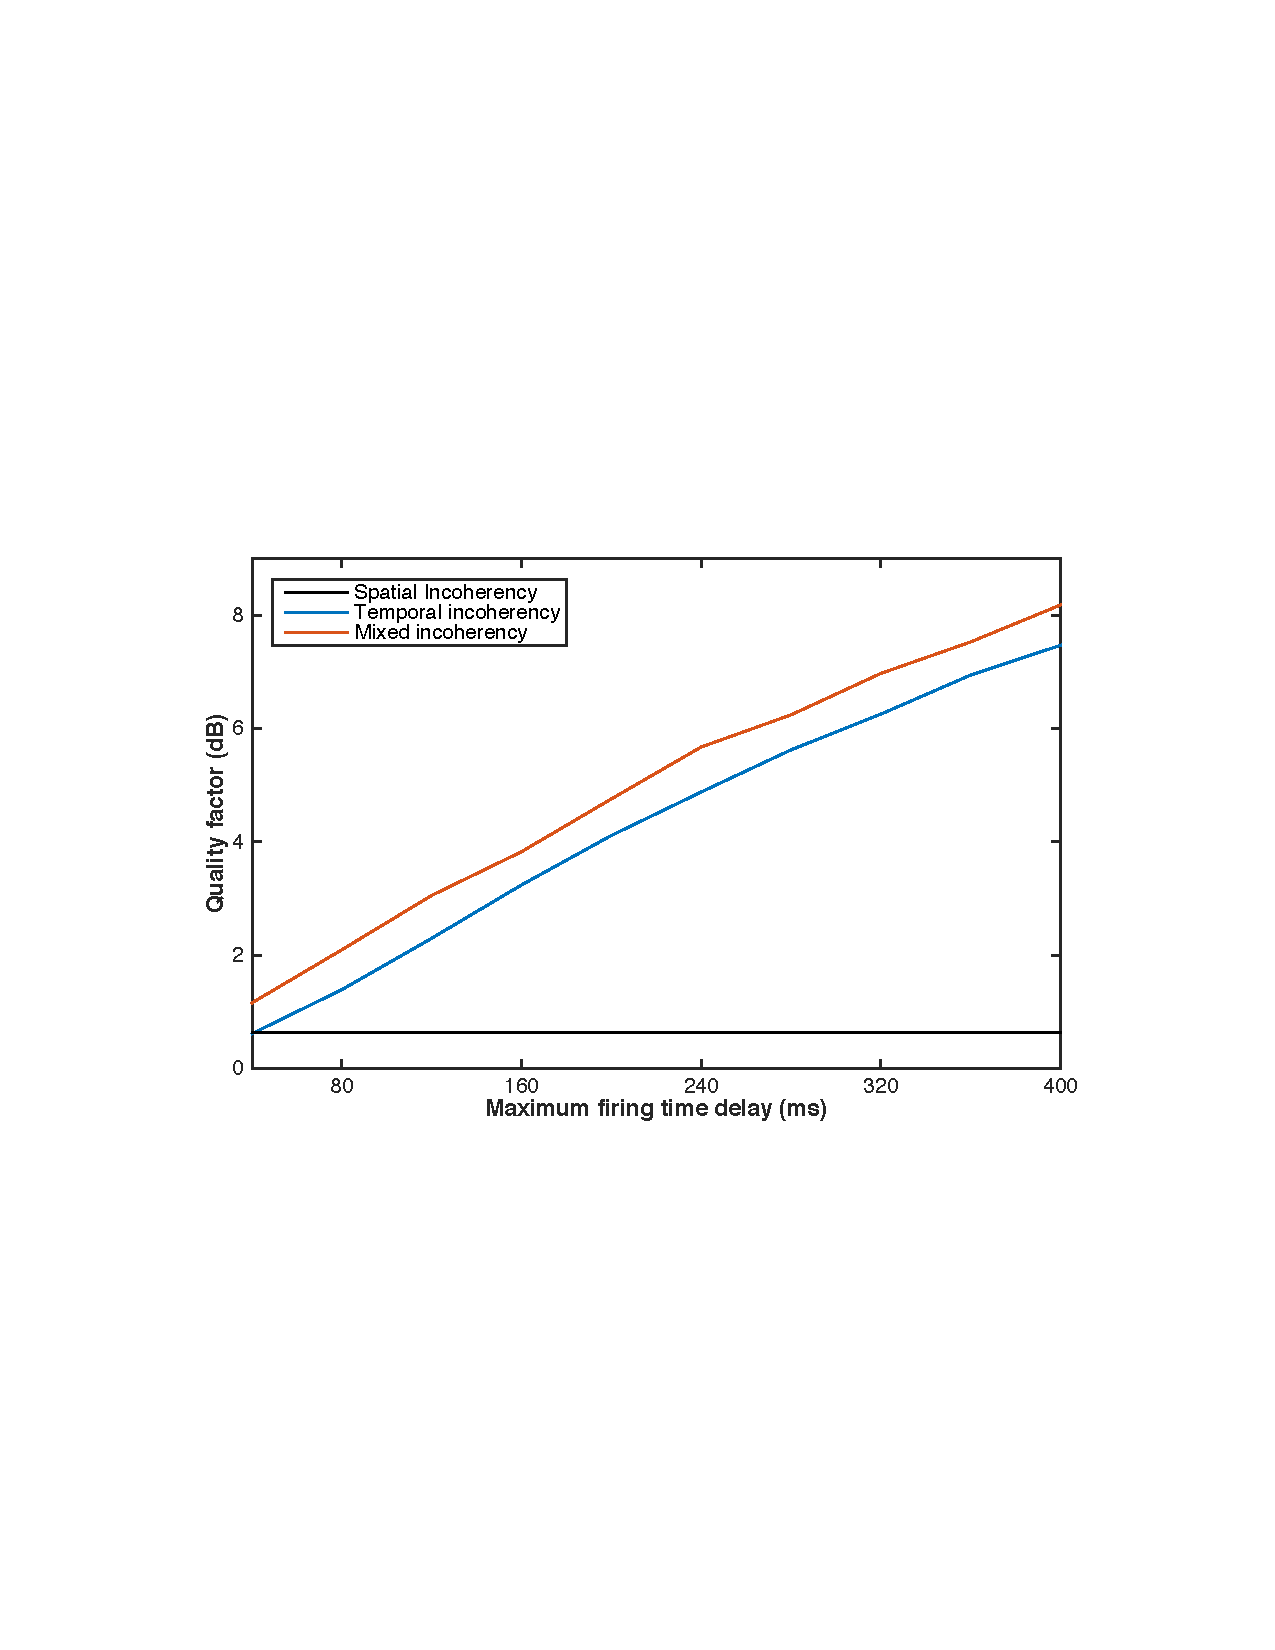
\includegraphics[width = 0.6\textwidth]{Plots/BlendingPatterns/quality_line_plot_avg}
	\caption{The 3 suggested blending patterns are simulated with maximum firing time delays between \SI{40}{\milli\second} and \SI{400}{\milli\second}. The quality factors are computed with respect to the unblended data and illustrated as a function of the maximum firing time.}
	\label{fig:Ch-Results-QualityFactors}
\end{figure}

\todo[inline]{For the conclusion/discussion of these results: \\ 
				Say that a high degree of incoherency is required for successful deblending, but it is not useful as a control factor of the deblending performance. Instead the maximum firing time delay allows to fine tune the quality factor and might be suitable to fine tune a trade off between deblending quality and acquisition time.\\
				One can also say that the  spatial incoherency performs poorly because its degree of incoherency is simply too low.}
				
				
				

\FloatBarrier
\section{$f$-$k_x$-$k_y$ Filter vs. $f$-$k_{(x)}$ Filter}

The 3D $f$-$k_x$-$k_y$ filter removes incoherent energy in the crossline and inline direction. The suggested 3D blended acquisition design blends sources within the same crossline. Hence, the question arouses whether an extension of the 2D $f$-$k_x$ filter to the inline direction provides significant deblending enhancements.

For this purpose the synthetic data of Figure \ref{fig:Ch-Results-Unbl-Delphi} is blended: Within each crossline there are 21 sources, which are blended in 3 experiments. For each experiment 7 randomly selected sources are blended with random time delays, i.e. the blending pattern with mixed incoherency is applied. The maximum allowed firing time delay is set to \SI{400}{\milli\second}. 

The blended data is deblended with the 3D deblending algorithm. In the one case a 2D $f$-$k_x$ filter is applied (see Figure \ref{fig:Ch-Results-Deblending-2dfk}). In the other case a 3D $f$-$k_x$-$k_y$ filter is applied (see Figure \ref{fig:Ch-Results-Deblending-3dfk}). It is clearly visible that the deblending quality increases significantly with the 3D $f$-$k_x$-$k_y$ filter.

In order to quantify the quality gap between the results with 2D and 3D filters, the plot in Figure \ref{fig:Ch-Results-QualityFactors} is reproduced with a 2D $f$-$k_x$ filter (see Figure \ref{fig:Ch-Results-QualityFactors_2d}).
\todo[inline]{The Matlab code for this test is prepared but it takes very long time. I will let it run over night. The quality factors are expected to be about half of the quality factors for the 3D fkk filter.}
 
\begin{figure}
	
	\centering
	\begin{subfigure}[t]{0.8\textwidth}
		\includegraphics[width = \textwidth]{Plots/2dvs3dfk/Deblendedv6_xt_100}
		\caption{}
		\label{fig:Ch-Results-Deblending-2dfk}
	\end{subfigure}
	
	\par\bigskip
	
	\centering
	\begin{subfigure}[t]{0.8\textwidth}
		\includegraphics[width = \textwidth]{Plots/2dvs3dfk/Deblendedv5_xt_100}
		\caption{}
		\label{fig:Ch-Results-Deblending-3dfk}
	\end{subfigure}
	
	\caption{}
	\label{fig:Ch-Results-Deblending-2dvs3d-fk}
\end{figure}

\begin{figure}
	\centering
	\includegraphics[width = 0.6\textwidth]{Plots/2dvs3dfk/Q_vs_tg_2dfk}
	\caption{}
	\label{fig:Ch-Results-QualityFactors_2d}
\end{figure}


\section{Feasibility}

The results demonstrate how the 3D deblending result can be optimized. In practice, the sources within a crossline must be fired and recorded before the vessel reaches the next inline position.

For this feasibility test it is assumed that the vessel moves with a speed of \SI{1.2}{\metre\per\second}, the recording time per experiment is \SI{3}{\second} and the maximum firing time delay is \SI{400}{\milli\second}. 

\begin{figure}
	\centering
	\includegraphics[width=0.7\textwidth]{Plots/Feasibility/acquisition-set-up}
	\caption{}
	\label{fig:Ch-Results-Feasibility-Set-Up}
\end{figure}







